%%
% The BIThesis Template for Undergraduate Proposal Report
%
% 北京理工大学毕业设计开题报告 —— 使用 XeLaTeX 编译
%
% Copyright 2020-2022 BITNP
%
% This work may be distributed and/or modified under the
% conditions of the LaTeX Project Public License, either version 1.3
% of this license or (at your option) any later version.
% The latest version of this license is in
%   http://www.latex-project.org/lppl.txt
% and version 1.3 or later is part of all distributions of LaTeX
% version 2005/12/01 or later.
%
% This work has the LPPL maintenance status `maintained'.
%
% The Current Maintainer of this work is Feng Kaiyu.
%
% This work consists of the files main.tex, misc/cover.tex and
% the external PDF misc/reviewTable.pdf
%
% Compile with: xelatex -> biber -> xelatex -> xelatex
%%

\documentclass[type=undergraduate_proposal]{bitreport}

\BITSetup{
  cover = {
    % Custom date.
    % date = 2022-08-08
  },
  info = {
    author = 傅泽,
    school = 计算机学院,
    major = 计算机科学与技术,
    class = 07111905,
    supervisor = 陆慧梅
% externalSupervisor = 向勇
  },
  misc = {
    reviewTable = misc/reviewTableBlank.pdf
  }
}

% Required by biber
\usepackage[style=gb7714-2015,backend=biber]{biblatex}
% Required by figure.
\usepackage{float,graphicx}
% Required by tables.
\usepackage{multirow}
\usepackage{makecell}

% 参考文献引用文件 refs.bib
\addbibresource{misc/refs.bib}

%%
% 文档开始
\begin{document}

\MakeCover

% 评审表
\MakeReviewTable

% 内容开始
\section{毕业设计(论文)选题的内容}
本课题基于实验室已有工作——基于区块链的出租车调度系统和树状区块链,对树状区块链的性能表现进行综合测试,研究树状区块链相较传统链式区块链的性能比较。课题首先研究树状区块链相较传统单链结构区块链的优势与局限性;其次,对实验室已有工作——基于区块链的出租车调度系统进行复现,验证其可用性;对于树状区块链引入的特色功能——跨子链转账,设计系统的性能测试,并建立简单的数学模型,对开发者在不同应用场景下对树状区块链和传统单链结构区块链的选择提供建议。在上述工作的基础上,以出租车调度系统为背景,测试树状区块链和传统链式区块链在运行该调度系统时的性能表现差异。最后,提出一种使用Rust编程语言重写树状区块链的可行方案,讨论将现有树状区块链的开发平台由以太坊开发平台迁移至更加优秀Substrate开发框架的优势及可行性,并进行部分树状区块链的功能特性的重写工作加以佐证。

\section{研究方案}
\subsection{本选题的主要任务}
\begin{enumerate}
  \item 了解传统链式区块链的底层原理、工作机制,了解区块链和车联网技术在国内外发展的近况\cite{blockchainCurrent}\cite{iov},学习相关法律规定,以可持续发展的角度最大化区块链技术对人类的积极作用;
  \item 在导师指导下,阅读国内外中外文文献,自主学习相关知识,了解在本地网络搭建传统区块链与树状区块链私有链、智能合约的编写与部署等操作的方法。了解出租车调度系统的需求、工作原理,选择适量且适当的评估准则对系统性能表现进行衡量;
  \item 完成传统区块链和树状区块链的搭建,分别于其上完成智能合约的部署和运行测试;此后,根据要求2中选定的性能指标,对其进行性能测试;
  \item 学习Substrate区块链开发框架与以太坊开发平台的异同,并尝试利用Substrate对重写树状区块链进行重写工作,为Substrate区块链引入部分树状区块链的功能特性
  \item 完成毕业设计论文一份,开发成果软件一份,软件配套文档一份;
  \item 完成毕业设计英文翻译工作,训练跨文化交流的书面表达能力,为在非母语环境下进行学术相关沟通交流奠定基础;
\end{enumerate}

\subsection{技术方案的分析、选择}

% \begin{figure}[!ht]
%   \centering
%   \includegraphics[width=0.6\linewidth]{example-image-a}
%   \caption{Merge sort recursion tree:一张示意图}
%   \label{fig:mergesort}
% \end{figure}

\subsubsection{已有工作}
目前,实验室已有的工作实现了基于以太坊智能合约平台实现 geohash 矢量地图的存储与调用,并进一步实现了基于 geohash 的导航算法以及相应的车乘调度系统;同时,在区块链上运行的信誉评估系统也已经被提出。

GeoHash 是一种新型的地址编码方式, 由 Gustavo Niemeyer 和 G.M. Morton 发明\cite{geohash_intro},其优势在于:将传统的经纬度表示的地图数据表示为基于 geohash 编码的地图数据,并存储于区块链上,不仅得以将二维的位置信息以更方便索引的一维字符串形式存储,而且摆脱了对外部地图数据的依赖,保障了地图数据的安全性;同时, geohash 与传统经纬度坐标的转换也十分便捷\cite{7160068},有利于与已有项目进行对接。

在导航算法中,使用 A* 算法\cite{a_star},以道路长度作为计算因子。

在区块链上运行的信誉评估系统,可以对司机和乘客的行为习惯等方面进行评分,供司机接单,乘客下单提供参考。由于摆脱了中心服务器的限制,可以保证了数据稳定性,提高了数据可信度,进而提升出行乘车的总体体验。

在此基础上,多点并发的车程调度系统,多司机、多乘客的调度与路径导航等功能得以实现。

\subsubsection{计划进行的测试工作}
传统的区块链结构是单链结构,其要求所有节点必须处于同一条链上,面对车联网数以万计,甚至更多的节点数量,传统区块链的查询效率等问题势必将成为性能瓶颈之一\cite{limits}。

为满足车联网所需的性能要求,有效利用地理分区的特性,实验室提出了一种称为“树状区块链”的概念\cite{sensors}。传统区块链中,每个区块的结构都大致相同。树状区块链则创新地提出,使用三种不同的区块,利用地理分区的特性将单链结构改造为树状结构。其示意图如 \ref{fig:tree-like-blockchain} 所示。

\begin{figure}[!ht]
  \centering
  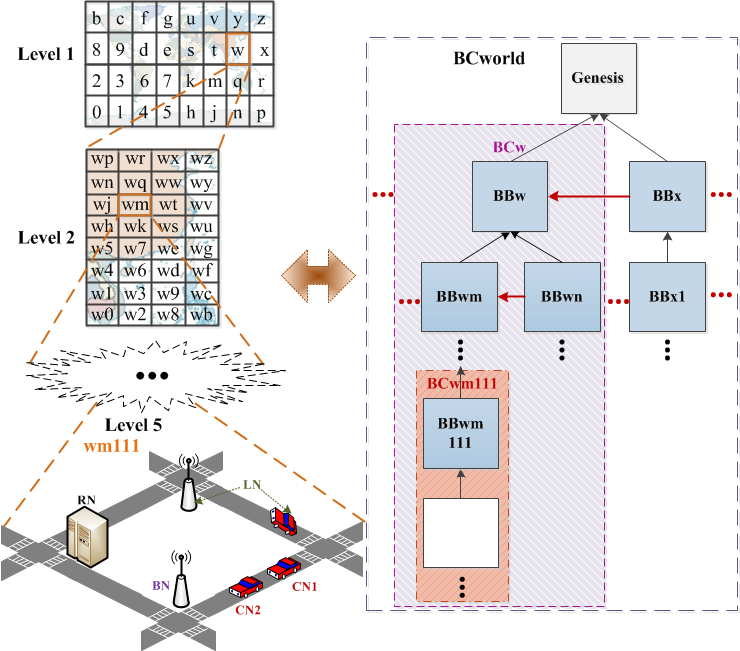
\includegraphics[width=0.6\linewidth]{misc/tree-like-blockchain.png}
  \caption{树状区块链示意图}
  \label{fig:tree-like-blockchain}
\end{figure}

\ref{fig:tree-like-blockchain} 中展示了树状区块链的大致构造。与传统区块链不同,树状区块链由创世区块 Genesis ,分支区块 Branch Block (简称 BB ) 和普通区块 Common Block (简称 CB )组成。创世块是所有区块的根节点,分支区块以 geohash 作为索引,作为拥有相同的 geohash 前缀的其他区块的父节点;普通区块和传统区块链中的区块无甚不同,呈经典的单链结构。

以geohash前缀作为索引的特性,允许树状区块链以较高的效率对各个节点进行索引,在继承了区块链高安全性的同时,也兼顾了效率;然而,上述结构带来的便捷也并非毫无代价。当节点的地理位置发生较大移动时,必须要考虑将节点进行跨链移动,以维持查找的正确性。换言之,树状区块链需要正确地构建父链结构,并维持多链间的信息同步。

本项目旨在选定指标,基于实验室已有的,有关出租车调度的工作,对传统区块链和树状区块链的性能表现进行测试,验证树状区块链在基于geohash进行索引时的理论优越性,以及为实现如此优越性所可能要付出的性能代价。

\subsubsection{区块链在不同语言上的实现}
目前,实验室所使用的搭建私有区块链的工具乃是基于Golang写成的工具Go-Ethereum\cite{about_geth}(下称Geth)。Geth是以太坊官方发布的一组工具,用于开发和接入可在以太坊上运行的千千万万的基于区块链构建的应用程序,有着大量的用户群体和完善的工具链体系。

然而,在一些开源操作系统的数据存储过程上使用区块链以加强数据安全性的尝试并不能完全依赖Geth。得益于Rust编程语言对于内存安全的强有力的保证\cite{system_programming},绝大多数开源操作系统都正基于这一新兴的语言进行开发。为令操作系统与区块链更好、更深度地融合,基于Rust编写的Substrate横空出世\cite{about_substrate},其具有灵活小巧的特点,非常适合在Rust环境下进行区块链开发。本课题将提出一种使用Rust编程语言重写树状区块链的可行方案,讨论将现有树状区块链的开发平台由以太坊开发平台迁移至更加优秀Substrate开发框架的优势及可行性,并进行部分树状区块链的功能特性的重写工作加以佐证。

\subsection{实施技术方案所需的条件}

目前选定的,用于构建区块链和辅助进行测试的软硬件工具如 \ref{tab:soft-hardware} 所示。

\begin{table}[!ht]
  \centering
  \caption{硬件、软件环境}
  \label{tab:soft-hardware}
  \begin{tabular}{@{}lcl@{}}
    \toprule
                          & 指标      & \multicolumn{1}{c}{版本参数}                \\
    \midrule
    \multirow{2}{*}{硬件环境} & CPU     & Intel i7-9750H                          \\
    \cmidrule(l){2-3}     & RAM     & 24 GB                                   \\
    \midrule
    \multirow{5}{*}{软件环境} & 操作系统    & \begin{tabular}[c]{@{}l@{}}
                                        Windows 10 64位专业版 \\  Ubuntu 22.04.1 LTS
                                      \end{tabular} \\
    \cmidrule(l){2-3}
                          & Python  & 3.10.6                                  \\
    \cmidrule(l){2-3}
                          & Node.JS & 18.12.1                                 \\
    \cmidrule(l){2-3}
                          & npm     & 8.19.2                                  \\
    \bottomrule
  \end{tabular}
\end{table}

\subsection{存在的主要问题和技术关键}
目前存在的主要问题是:尚需更加深入地理解树状区块链和普通传统区块链的不同,明确其达到更好性能的实现方法和相比起传统区块链的开销,并以此为依据,设计测试用例,证明其相比传统区块链在车联网领域更具有应用前景的设想。

为实现以上目标,需要选择并熟练使用构建并管理树状区块链的工具,辅助测试进行的自动化测试工具等。项目相关的关键技术如下表所示。

\begin{table}[!ht]
  \centering
  \caption{关键技术}
  \label{tab:key-tech}
  \begin{tabular}{@{}lcl@{}}
    \toprule
    用途         & 相应技术                  \\
    \midrule
    构建和管理树状区块链 & Geth,Substrate        \\
    \midrule
    自动化管理树状区块链 & TypeScript,JavaScript \\
    \midrule
    自动化测试和辅助处理 & Python                \\
    \midrule
    构建和编辑Substrate框架 & Rust \\
    \bottomrule
  \end{tabular}
\end{table}


\subsection{预期能够达到的研究目标}
本项目旨在选定指标,基于实验室已有的,有关出租车调度的工作,对传统区块链和树状区块链的性能表现进行测试,验证树状区块链在基于geohash进行索引时的理论优越性,以及为实现如此优越性所可能要付出的性能代价。除此以外,本项目还将就数个性能指标进行优化,对目前已有的树状区块链及其有关出租车调度的应用加以改进;并将其从以太坊迁移到Substrate上。

课题预期达到以下目标:
\begin{itemize}
  \item 成功复现实验室已有工作——基于区块链的出租车调度系统;
  \item 对于树状区块链引入的特色功能——跨子链转账,设计系统的性能测试,并建立简单的数学模型,对开发者在不同应用场景下对树状区块链和传统单链结构区块链的选择提供建议;
  \item 以出租车调度系统为背景,测试树状区块链和传统链式区块链在运行该调度系统时的性能表现差异;
  \item 提出一种使用Rust编程语言重写树状区块链的可行方案,讨论将现有树状区块链的开发平台由以太坊开发平台迁移至更加优秀Substrate开发框架的优势及可行性,并进行部分树状区块链的功能特性的重写工作加以佐证。
\end{itemize}

完成毕业设计论文一份,开发成果软件一份,软件配套文档一份,以及毕业设计英文翻译工作。

\section{课题计划进度表}
大致的课题计划进度如表 \ref{tab:progress} 所示。

\begin{table}[!ht]
  \centering
  \caption{毕业设计计划进度表}
  \label{tab:progress}
  \begin{tabular}{lp{4cm}p{4cm}p{3cm}}
    \toprule
    阶段 & \multicolumn{1}{c}{任务}      & \multicolumn{1}{c}{完成标志}        & 时间规划    \\ \midrule
    1  & 了解区块链基本原理和工具的使用             & 成功搭建本地私有链,并利用RPC进行交互操作          & 第1-2周   \\ \midrule
    2  & 了解树状区块链和传统区块链的区别,并学习部署合约的方法 & 基于实验室已有工作成果,在传统和树状区块链上部署智能合约    & 第3-6周   \\ \midrule
    3  & 挑选性能指标并对两个已搭建的链进行性能测试       & 形成详细测试报告,对比两种链在不同指标上的表现异同       & 第7-10周  \\ \midrule
    4  & 尝试将树状区块链的部分功能特性使用Rust重写,并应用到Substrate上  & 对重写的功能特性进行可用性测试,验证工作正确性 & 第11-14周 \\ \midrule
    5  & 依照工作进度,形成毕业设计论文,同步进行翻译工作    & 成功完成毕业设计                        & 第1-14周  \\ \bottomrule
  \end{tabular}
\end{table}

\section{参考文献}
% 删除默认的「参考文献 / Reference」标题,使用上面定义的 section 标题
\printbibliography[heading=none]

\end{document}
